\section{evaluation}
\label{sec:eval}

We measured various performance aspects of Camelot to measure its
scalability and competitiveness with existing data processing
platforms. We developed a set of benchmark programs with diverse
memory access patterns, to measure the quality of our page eviction
strategies, threading performance, and raid overhead.

\subsection{Experimental setup}
Our tests were performed in the Mininet~\cite{mininet} as well as on real hardware.
Mininet is a host-local network emulator intended to rapidly prototype SDN and data center network environments. Mininet allow us to verify and deploy code quickly, without having to worry about hardware constraints or configuration. While absolute performance may not exactly be accurate, relative improvements are generally reliable. 
Our real hardware setup consisted of three servers, each of which equipped with a 10-Gigabit X540-AT2 NIC, 32 GB of memory, and two four-core Intel(R) Xeon(R) E5-2407 v2 CPUs. The cores do not support hyperthreading.
The microbenchmarks and threading tests were performed on real hardware to provide an accurate picture of the current system efficiency. The remaining tests were run in Mininet, as absolute performance was not of concern.

\todo{Stew, Bronson do you want to fill in your parts?}
\subsection{Threading Performance}
To understand the implications of multithreading, and to verify the functionality of our current networking stack, we conducted several microbenchmarks. We pinned each thread to one core in a round-robin fashion, as this approach has proven itself to be more stable and reliable during testing. Our benchmark consisted of a million read and write requests, which we then scaled up to 64 threads. The results are shown in Fig~\ref{fig:threads}.
As expected, throughput scales linearly up to eight threads and latency does not increase. Unfortunately, the program is unable to exhaust the NIC bandwidth, which is caused by a lack of request batching and the use of slow kernel networking code.

We decided to go beyond the expected scaling of eight cores and explore the system behaviour up to 64 threads. The pinned experiment ran stable, demonstrating a reasonable reliability. The throughput results exhibit a sawtooth pattern, with a local maximum occurring  every eighth thread. This pattern is caused by the number of cores and pinning. However, this does not explain the maxima achieved by 16 and 24 threads. We assume that these may be caused by batching of requests in the NIC buffer, which is beneficial for throughput.
Latency behaves as expected, with a mild increase in early iterations that transitions into wild instability the more threads are added.

\begin{figure*}[h]
    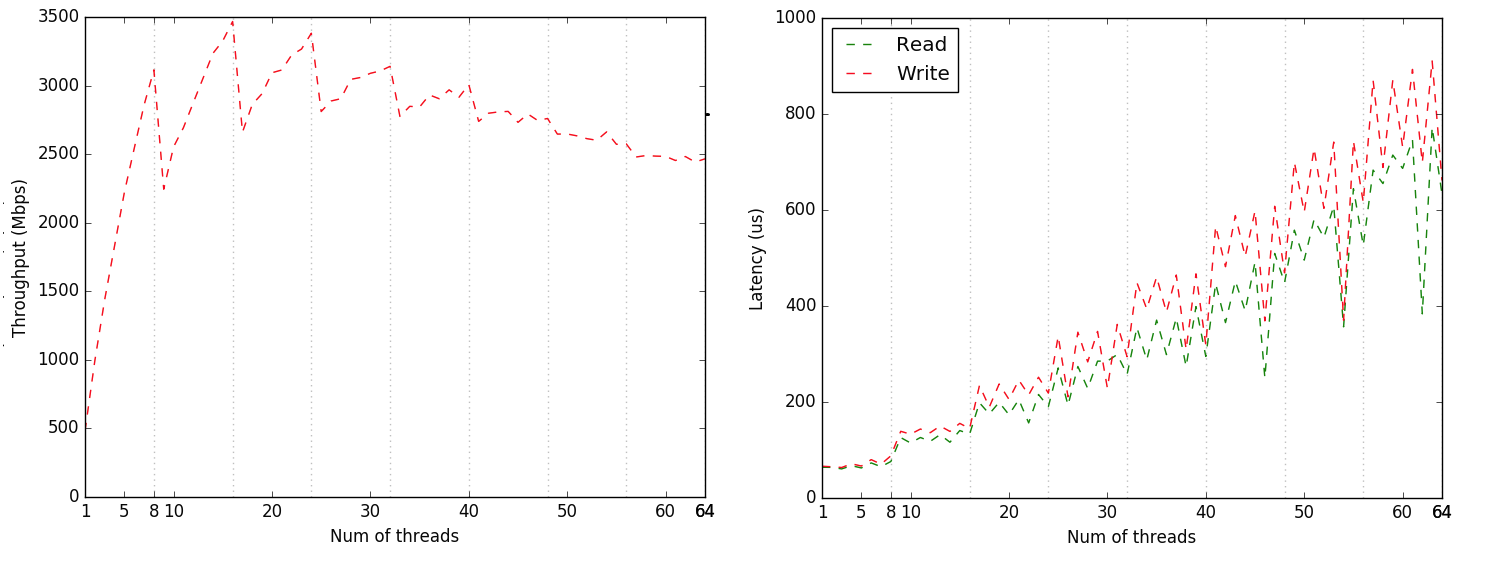
\includegraphics[width=\textwidth]{fig/threads_pinned}
    \caption{Microbenchmarks of the Camelot request API. The two figures show latency and throughput with threads pinned to cores in round-robin fashion.}
    \label{fig:threads}
\end{figure*}

\subsection{Paging Performance}
\todo{Bronson}

\begin{figure}[H]
    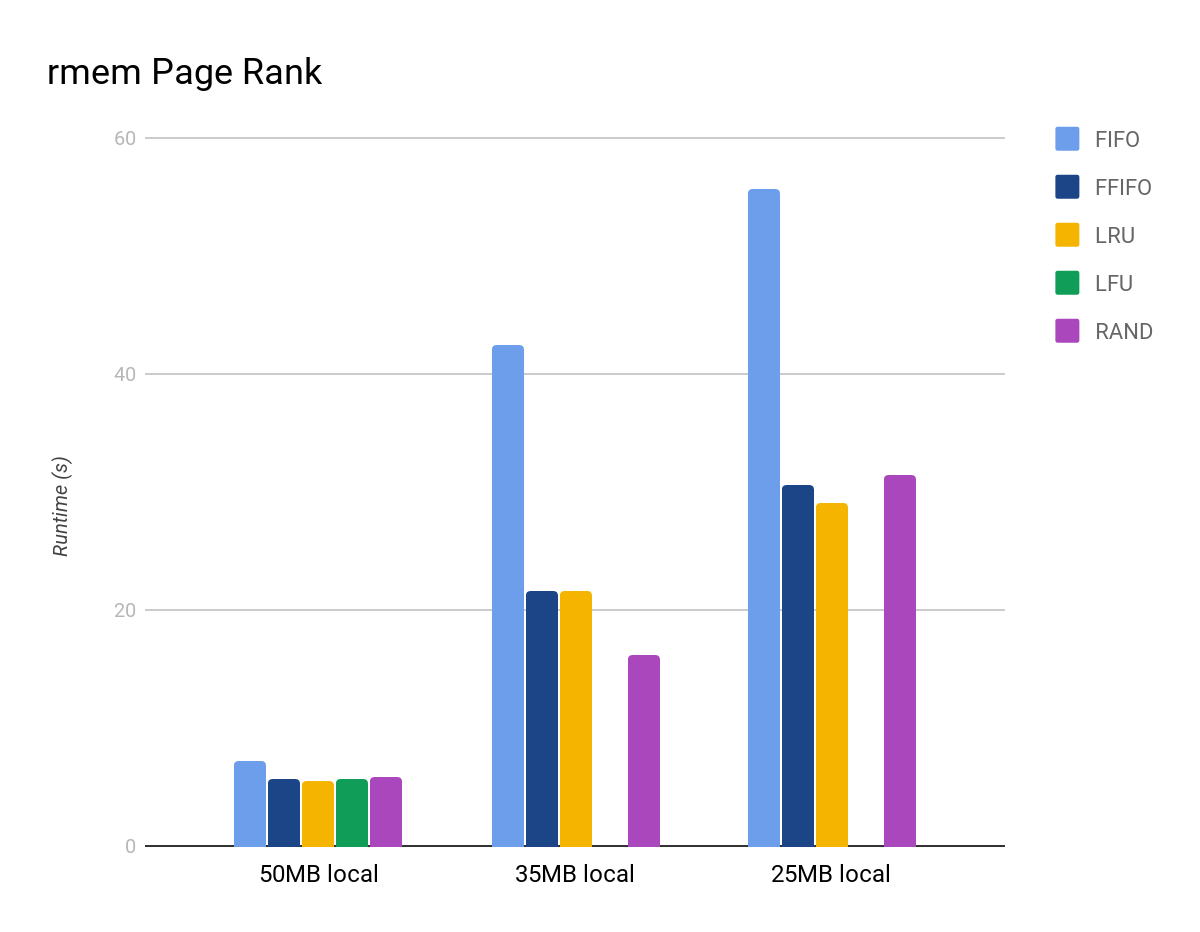
\includegraphics[width=\columnwidth]{fig/policyPerformance}
    \caption{\todo{Bronson}}
    \label{fig:policyPerformance}
\end{figure}

\begin{figure}[H]
    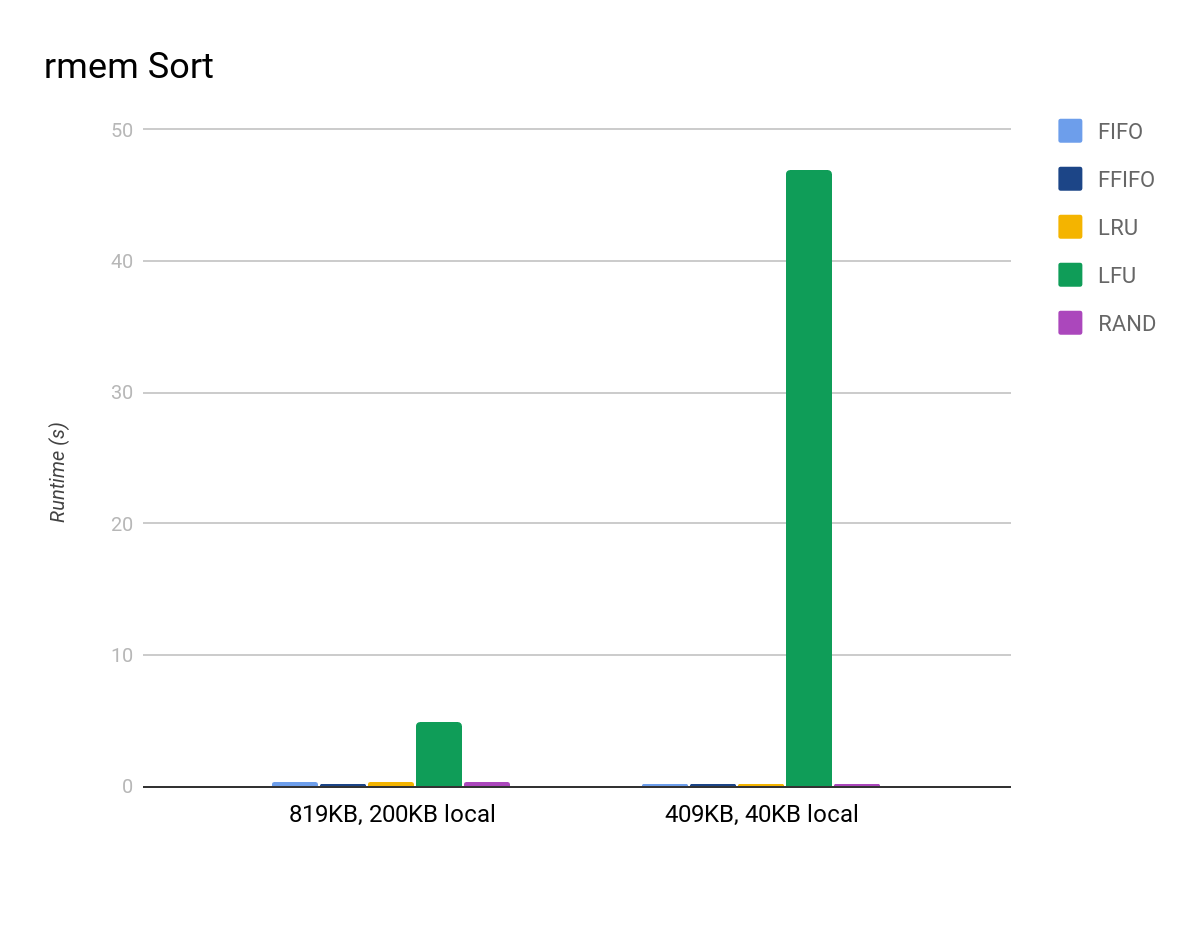
\includegraphics[width=\columnwidth]{fig/sortPerformance}
    \caption{\todo{Bronson}}
    \label{fig:sortPerformance}
\end{figure}

\subsection{RAID Overhead}
\todo{Stewart}

\begin{figure}[H]
    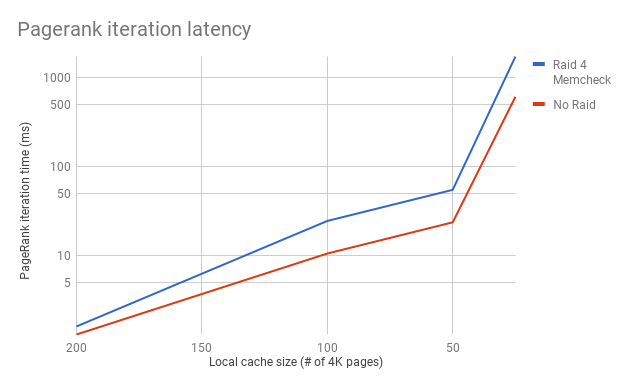
\includegraphics[width=\columnwidth]{fig/Raid4Overhead}
    \caption{\todo{Stewart}}
    \label{fig:raid4Overhead}
\end{figure}

\begin{figure}[H]
    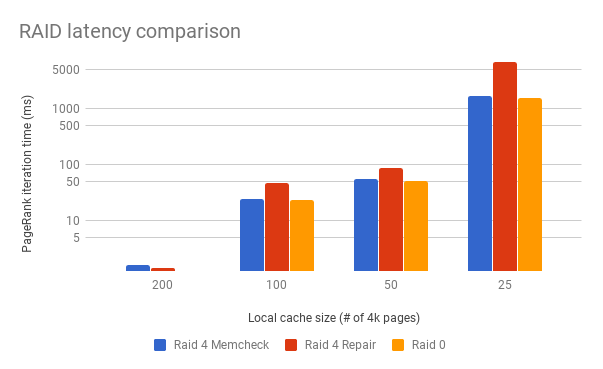
\includegraphics[width=\columnwidth]{fig/RaidComparison}
    \caption{\todo{Stewart}}
    \label{fig:RaidComparison}
\end{figure}

